\documentclass[twocolumn, 10pt]{asme2ej} %TODO: use IEEEtran document class
                                         %instead
\usepackage{epsfig}
\usepackage{hyperref}
\usepackage{graphicx}
\graphicspath{ {images/} }
\usepackage{multirow}
\usepackage{array}
\usepackage{subcaption}

\title{Artifice: Generalized Object Detection in Scientific Images}

\author{Benjamin Killeen
  \affiliation{
    \href{mailto:killeen@uchicago.edu}{killeen@uchicago.edu}
  }
}

\author{Gordon Kindlmann \affiliation{
    \href{mailto:glk@uchicago.edu}{glk@uchicago.edu}
  }
}

\begin{document}
\maketitle

\begin{abstract}
  {\it Together with large training sets, Deep Neural Networks (DNNs) have
    enabled a wide range of advancements in Computer Vision tasks, especially
    with regard to object detection in real-world images. Object detection for
    scientific images, on the other hand, presents challenges unlike more
    traditional vision tasks. First, experiments exhibit a scarcity of labelled
    data, a problem which we address through active learning and data
    augmentation. Second, scientific experiments involve inherent constraints,
    such as a natural law or governing principle, which the experimenter intends
    to observe. Although this quality seems advantageous for data augmentation,
    it threatens to undermine the scientific rigor of DNNs for laboratory
    tasks. In this progress report, we describe our ongoing effort toward
    training DNNs which are agnostic to inherent constraints yet perform
    reliably on scarce data.\footnote{Code available at
      \href{https://github.com/bendkill/artifice}
      {github.com/bendkill/artifice}}}
\end{abstract}

\section{Introduction}
\label{sec:introduction}

Imaging systems are a vital component of many scientific experiments, used as
the primary measuring device of properties such as object location and
orientation. In cases where no alternative measuring device exists, accurate
labeling is of the utmost importance. However, such image analysis can prove
labor-intensive. Traditional methods involve \emph{ad hoc} solutions suited for
one experimental setup, even though more general object detection tasks have
been well-studied in Computer Vision. \cite{bernardis_finding_2010} uses a
graph-cut approach for dot localization, noting various scientific applications,
and \cite{ronneberger_u-net:_2015} applies a DNN for semantic segmentation of
neuronal structures in electron microscope stacks. In this report, we introduce
\emph{Artifice}, an ongoing effort to generalize across scientific tasks using
DNNs.

Deep Neural Networks (alternatively, deep convolutional neural networks) have
shown remarkable success on real-world tasks \cite{krizhevsky_imagenet_2012}, as
defined by datasets like ImageNet \cite{deng_imagenet:_nodate} and COCO
\cite{lin_microsoft_2014}. These and other data underlie supervised learning
approaches for increasingly complex systems, such as self-driving
vehicles. Fig. \ref{fig:traditional-graph} shows a high-level outline of
supervised learning for computer vision. Scientific experiments, on the other
hand, have no dataset except what they generate; each experiment constitutes its
own unique vision task. Artifice addresses this scarcity of labeled data through
active learning \cite{settles_active_2012, kao_localization-aware_2018,
  jain_active_2016} and data augmentation \cite{krizhevsky_imagenet_2012,
  ronneberger_u-net:_2015}. It also confronts a problem unique to scientific
tasks, which we refer to as inherent constraints.

Unlike real-world tasks, scientific tasks aims to capture some natural law or
governing principle in the data. Images of a sphere in free-fall, for example,
capture the acceleration of gravity; a video of ants hunting for food obeys
simple rules governing swarm behavior. These principles constitute
\emph{inherent constraints}: patterns in the dataset reflecting the subject of
scientific inquiry itself. They differ from \emph{imposed constraints}, which
the experimenter controls. The experiment shown in fig. \ref{fig:gyros}, for
example, constrains each moving dots to a circular region.

We distinguish between imposed and inherent constraints for the purpose of
training. Because imposed constraints reduce the vision task, Artifice
incorporates them into its data augmentation step, as in
Fig. \ref{fig:artifice-graph}. Crucially, imposed constraints are
well-parameterized and guaranteed; the experimenter builds them into the vision
task. Inherent constraints offer a similar advantage, since one could simulate
their effects to further augment training data, but \emph{doing so could violate
  the scientific method}. The experimenter cannot anticipate inherent
constraints in order to build a better measuring stick, so to speak, because
scientific experiments require unbiased measurement. Even the initial dataset,
before any augmentation, contains inherent constraints that could influence
training. As much as possible, Artifice aims to be agnostic to these constraints.

\begin{figure*}
  \centering
  \begin{subfigure}{0.4\linewidth}
    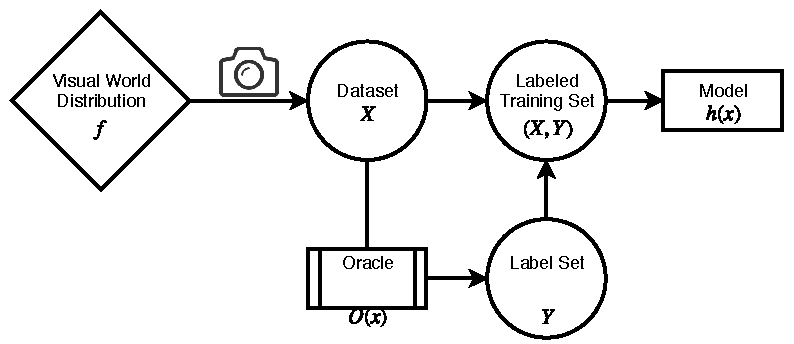
\includegraphics[width=\columnwidth]{traditional_graph}
    \caption{Traditional dependency graph}
    \label{fig:traditional-graph}
  \end{subfigure}
  \hspace{0.1\linewidth}
  \begin{subfigure}{0.4\linewidth}
    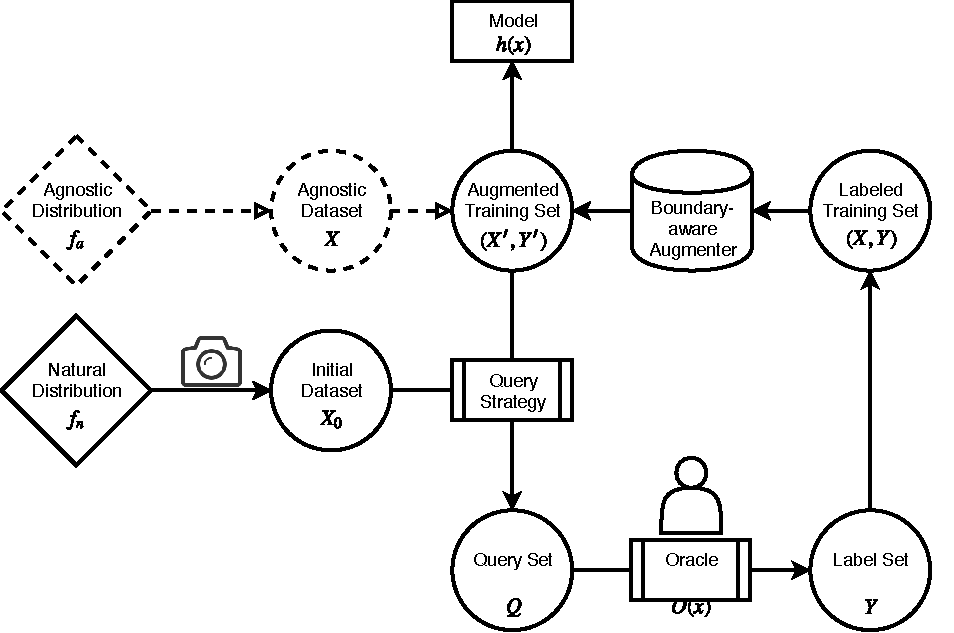
\includegraphics[width=\columnwidth]{artifice_graph}
    \caption{Artifice's dependency graph}
    \label{fig:artifice-graph}
  \end{subfigure}
  \caption{For a traditional vision task \textbf{(a)}, a camera converts
    real-world \textit{scenes} into an unlabeled dataset $X$. These scenes have
    actual attributes $\tilde{Y}$ which a \textit{labeller} records as the
    ``ground truth'' or ``measurement'' $Y$. A classifier or regression model
    $f$, trained on $(X,Y)$, produces predictions $\hat{Y}$.\\
    Artifice's dependency graph \textbf{(b)}, specialized for scientific vision
    tasks, distinguishes between two types of constraints. \textit{Imposed
      constraints}, such as physical boundaries, are known to the experimenter,
    but \textit{inherent constraints}, such as a physical law, are the subject
    of inquiry. \textit{Adverse noise}, including lighting changes or object
    deformation, also influences the experiment. In \textbf{(b)}, the augmented
    dataset $X$ is continually updated by the Training Cycle. A
    \textit{selector} chooses the query set $Q \subseteq X'$ based on existing
    predictions $\hat{Y}$. A \textit{labeler} produces imperfect ground truth
    $Y$, which enables the \textit{augmenter} to intelligently update the
    dataset $X'$, incorporating imposed constraints. Here, dashed lines
    represent single instance connections, such as instantiating $X' \gets X$,
    rather than continual dependency throughout the Training Cycle.}
  \label{fig:dependency-graphs}
\end{figure*}

\section{Related Work}
\label{sec:related-work}

The problems of data scarcity and biases are well-considered in computer
vision. \cite{torralba_unbiased_2011} explores bias in popular datasets for
computer vision by training DNNs on one dataset but testing them on another
(employing a test-train split for fairness). Unsurprisingly, networks perform
best on the dataset for which they were trained, even though datasets like
ImageNet aim to capture the unbiased visual world. Creating unbiased datasets
for real-world vision tasks remains an open problem, one which may demand a
reckoning for the community's focus on improving dataset performance scores.

\cite{ronneberger_u-net:_2015} describes a novel segmentation architecture using
up-convolutions which, paired with their data augmentation scheme, performs well
on biomedical images taken from electron stacks. Like Artifice,
\cite{ronneberger_u-net:_2015} confronts data scarcity but also focuses on
applications in biomedical imaging, where semantic segmentation is often
sufficient. Artifice aims to address scientific tasks more generally, using
semantic segmentation as one component of a general detection system, capable of
recovering location, orientation, or shape for multiple objects. Capturing these
quantities with minimal human effort would accelerate a wide range of scientific
experiments.


\begin{figure}
  \centering
  \begin{subfigure}{0.4\linewidth}
    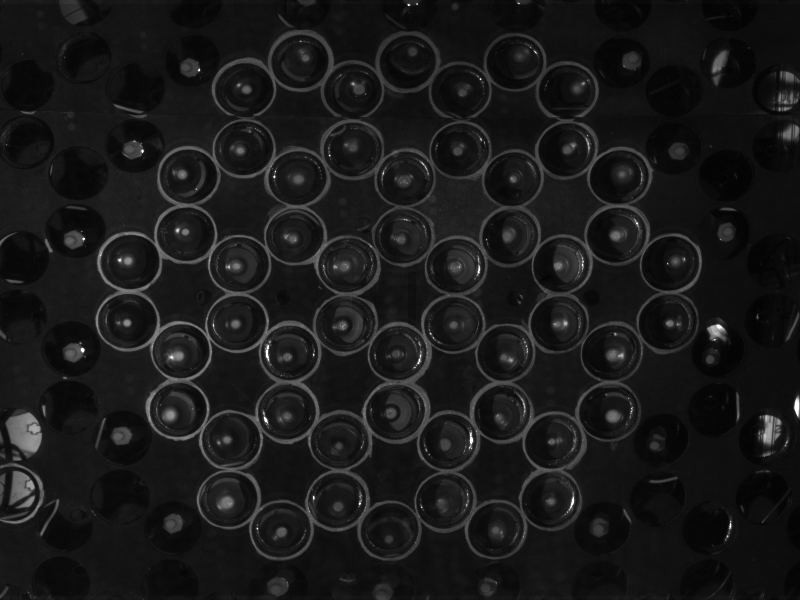
\includegraphics[width=\linewidth]{gyros}
    \caption{Gyroscopic model}
    \label{fig:gyros}
  \end{subfigure}
  \hspace{0.1\linewidth}
  \centering
  \begin{subfigure}{0.4\linewidth}
    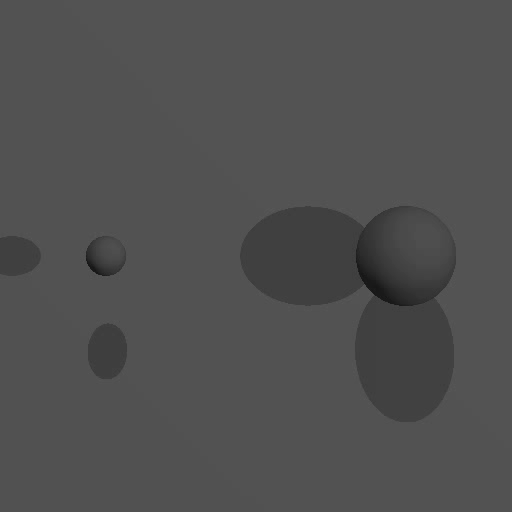
\includegraphics[width=\linewidth]{coupled_spheres}
    \caption{Coupled spheres}
    \label{fig:coupled-spheres}
  \end{subfigure}

  \caption[example experiments]{Example images from scientific experiments:
    \textbf{(a)} gyroscopic model for topological metamaterials
    \cite{nash_topological_2015}. Each dot is constrained to the circle
    surrounding it. \textbf{(b)} still frame from a simulated experiment of two
    spheres coupled by an invisible spring. Full video \href
    {https://github.com/bendkill/artifice/blob/master/docs/coupled_spheres.gif}
    {here}.}
  \label{fig:example-experiments}
\end{figure}

\section{Simulated Experiments}
\label{sec:simulated-experiments}

In order to show Artifice's effectiveness, we develop several virtual
experiments. These simulations offer several advantages over images from real
experiments, such as in Fig. \ref{fig:gyros}. First, we have perfect knowledge
of the experiment's ``Truth'' $\tilde{Y}$, as opposed to imperfect measurements,
or ``ground truth,'' $Y$. In well established datasets, $\tilde{Y}$ and $Y$ are
nearly identical, but Artifice must rely on one or a few human labelers for what
should be unambiguous quantities. For testing, we calculate $\tilde{Y}$ from the
known parameters of the simulation, and we emulate a human labeler by
introducing small perturbations to $\tilde{Y}$, producing $Y$. Part of
Artifice's goal is to train a DNN with predictions $\hat{Y}$ that more closely
approximate $\tilde{Y}$ than the labels $Y$. Simulated experiments allow us to
test this performance.

Fig. \ref{fig:coupled-spheres} shows one such experiment. In this case, two
spheres with different masses rotate in free space, coupled by an invisible
spring. The goal of the Coupled Spheres experiment is to recover physical
properties of the spring using $(x,y)$ positions of the two spheres. Imposed
constraints include the $z$-coordinate of each sphere, which is set to the
image-plane, as well as each sphere's apparent size. Inherent constraints
include the physical properties of the spring, \textit{e.g.} the spring constant
and relaxed length. Adverse noise, which in this case includes any shadows,
lighting effects, and possible occlusion, also presents a challenge for
detection.

To demonstrate Artifice's resilience to inherent constraints, we intend to train
a DNN on one experiment and evaluate its performance on experiments with
different simulated springs. This simple example illustrates the general
resilience that we wish to develop.

\section{Method}
\label{sec:method}

Fig. \ref{fig:artifice-graph} shows Artifice's training scheme at a
high-level. The details of this scheme are an area of active inquiry, with open
questions pertaining to the \emph{selector}, for active learning; the
\emph{augmenter}, which should incorporate the experiment's imposed constraints;
and the model $f$, which employs one or more DNNs.

Because of the variety of scientific tasks, $f$ must remain flexible with regard
to its output. Toward this end, we envision a two-step procedure which (1)
obtains an instance segmentation \cite{ronneberger_u-net:_2015, bai_deep_2016}
for objects of interest and (2) learns the target parameters (location,
orientation, etc.) for each object. Whether these steps occur in an end-to-end
fashion or are divided between several training steps is an open question. We
do, however, consider (1) to be a vital step for the sake of maintaining
generality. Even in scientific tasks where segmentation is unneeded, such as the
Coupled Sphere experiment in \ref{sec:method}, obtaining pixel-level masks of
each object enables more advanced data augmentation methods.

Because we wish to minimize the man-hours required for training as much as
possible, Artifice uses an active learning scheme to select a query set
$Q \subseteq X'$ which will most inform training. The application of active
learning to semantic segmentation has received relatively little attention, with
the exception of \cite{vezhnevets_active_2012}, and the added complication of an
imperfect labeler remains an open question in the field
\cite{settles_active_2012}. Artifice aims to address both issues with its
\emph{selector}.

Finally, Artifice's \emph{augmenter} will incorporate both the semantic
segmentations obtained by $f$ and the imposed constraints specified by the
experimenter to improve training as much as possible. We hope to test many
augmentation methods while keeping in mind that the image space of a scientific
task is usually much more constrained than that of a real-world
task. \cite{krizhevsky_imagenet_2012}, for instance, uses sub-image extraction,
flipping, and PCA analysis of RGB channels to augment ImageNet. These methods are
not necessarily applicable to scientific tasks, where imposed constraints might
invalidate a flipped image, for instance.

\section{Conclusion}
\label{sec:conclusion}

We have outlined our ongoing efforts to develop Artifice, an object detection
scheme intended for scientific tasks. Much work remains to be done with regard
to Artifice's implementation, but we hope that by outlining our goals early, we
have elucidated some key problems unique to scientific tasks.

\begin{acknowledgment}
  Thanks to Michael Maire for input and guidance, as well as William Irvine for
  access to image data from his laboratory.
\end{acknowledgment}

\bibliographystyle{asmems4}
\bibliography{artifice}

\end{document}
%%% Local Variables:
%%% mode: latex
%%% TeX-master: t
%%% End:
